%====================================================================================================
\chapter{The ATLAS Experiment for HL-LHC} \label{ch:ATLASforHLLHC} 
%====================================================================================================
The ATLAS experiment is planned to upgrade in preparation for the HL-LHC. As the pile-up increases due to higher instantaneous luminosity, the event rate, including background event rate, will also rise. To cope with this, the detector will be enhanced to suppress backgrounds and maintain high resolution. This chapter introduces the components of the ATLAS detector relevant to this research-especially the muon spectrometer and the TDAQ system-and then outlines the planned upgrades to these subsystems for the HL-LHC.
%====================================================================================================
\section{Coordinate System} \label{sec:CoordinateSystem}
%====================================================================================================
To describe positions and directions of particles within the ATLAS detector, a right-handed Cartesian coordinate system is adopted with the origin located at the interaction point (IP). In this system, the \(x\)-axis points radially outward toward the center of the LHC ring, the \(y\)-axis points upward to the sky, and the \(z\)-axis follows the direction of the beam direction. 

Cylindrical coordinates \((\theta, \phi, z)\) are also commonly used. Here, \(\theta\) denotes the polar angle from the \(z\)-axis and spans from \(0\) to \(\pi\), while \(\phi\) is the azimuthal angle measured around the beam axis, ranging from \(-\pi\) to \(\pi\) from the \(x\)-axis. The distance from the \(z\)-axis is denoted by \(r\)(sometimes refered as \(R\)). A schematic of the coordinate system is shown in Figure~\ref{fig:ATLASCoordinate}.

\begin{figure}[htbp]
  \centering
  \includegraphics[width=1.0\textwidth]{figs/chapter2/ATLAS_coordinate.png}
  \caption{The coordinate system used in the ATLAS experiment \cite{mino}.}
  \label{fig:ATLASCoordinate}
\end{figure}

In the ATLAS experiment, since proton-proton collisions take place near the nominal IP, angular variables of produced particles are typically defined with respect to this point. While the polar angle \(\theta\), measured from the beam (z) axis, provides a direct geometric description, it lacks invariance under Lorentz boosts along the beam direction, making it less suitable for characterizing particle kinematics in high-energy collisions.
To overcome this, a variable called rapidity \(y\) is introduced. Rapidity \(y\) is defined in terms of a particle's energy and the momentum along \(z\)-axis, as in equation~\ref{eq:rapidity}. Its differences are invariant under boosts along the z-axis, making \(y\) it useful for comparing particle distributions across different frames:
\begin{equation}
  y = \mathrm{artanh}\, \beta_z = \frac{1}{2} \log \frac{E + p_z}{E - p_z},
  \label{eq:rapidity}
\end{equation}
where \(\beta_z\) is the velocity component normalized by the speed of light (in natural units) along the z-axis, \(E\) is the energy, and \(p_z\) is the momentum along the beam axis.

However, in most collider events, the final-state particles are highly relativistic, with masses negligible compared to their momenta. In such cases, rapidity \(y\) can be approximated by the pseudorapidity \(\eta\), which depends solely on the polar angle \(\theta\) and is thus easier to compute from detector measurements:
\begin{equation}
  \eta = -\log\left( \tan \frac{\theta}{2} \right).
  \label{eq:pseudorapidity}
\end{equation}

This \(\eta\) is widely used in physics analysis, as \(\eta\) retains the boost-invariant properties of \(y\) in the massless limit and being more convenient. In ATLAS experiment, the region of $|\eta| < 1.05$ is called \textit{endcap}, which consists of "A-side" and "C-side" corresponding respectively to the positive and negative directions of the \(z\)-axis. And the region between two endcaps, defined by $1.05 < |\eta| < 2.41$, is called \textit{barrel}.

In addition, transverse energy is defined as 
\[
  E_{\mathrm{T}} = E \sin \theta\,
\]
and transverse momentum as
\[
  p_{\mathrm{T}} = \sqrt{p_x^2 + p_y^2},
\]
which are also both widely used in physics analysis.

The angular distance \(\Delta R\) between two particles is a commonly used quantity, and is defined as
\begin{equation}
  \Delta R = \sqrt{(\Delta \eta)^2 + (\Delta \phi)^2}.
  \label{eq:deltaR}
\end{equation}
%====================================================================================================
\section{Magnet System} \label{sec:MagnetSystem}
%====================================================================================================
The ATLAS detector employs a unique hybrid magnetic system composed of four large superconducting magnets, and it spans 22~m in diameter and 26~m in length, with a stored energy of 1.6~GJ \cite{ATLASDetector2008}. This system includes a central solenoid and three toroidal systems (a barrel toroid and two endcap toroids), enabling high magnetic field coverage across both inner and muon detection systems.

The solenoid magnet, placed along the beam axis, provides a 2~T axial magnetic field for the Inner Detector (ID), optimized to minimize the radiative thickness in front of the electromagnetic calorimeter. Surrounding the calorimeter system are the toroidal magnets: the barrel toroid, composed of eight superconducting coils, and two endcap toroids, which together generate a toroidal magnetic field of about 0.5~T to 1~T for the muon spectrometer in the central and forward regions. The schematic geometry of the magnet windings is illustrated in Figure~\ref{fig:magnet_windings}. The solenoid is located inside the calorimeter volume, while the barrel and endcap toroids are interleaved around it. 

\begin{figure}[htbp]
  \centering
  \includegraphics[width=0.6\textwidth]{figs/chapter2/magnet_windings.png}
  \caption{Geometry of magnet windings and calorimeter steel. The eight barrel toroid coils and endcap coils are interleaved. The solenoid winding is located inside the calorimeter volume \cite{ATLASDetector2008}.}
  \label{fig:magnet_windings}
\end{figure}

%====================================================================================================
\section{Muon Spectrometer} \label{sec:MuonSpectrometer}
%====================================================================================================
The ATLAS muon spectrometer is the outermost subsystem of the detector, designed to provide independent momentum measurements for muons. It relies on magnetic deflection of muon trajectories using large superconducting air-core toroidal magnets we introduced in Section~\ref{sec:MagnetSystem} above.

The magnetic field in the spectrometer is shaped by a central barrel toroid and two endcap toroids. For muons with pseudorapidity $|\eta| < 1.4$, the bending power is provided mainly by the barrel toroid. In the forward regions ($1.6 < |\eta| < 2.7$), deflection comes from the endcap toroids. The intermediate transition region ($1.4 < |\eta| < 1.6$) receives contributions from both barrel and endcap fields. This field configuration creates a predominantly orthogonal bending force relative to the muon trajectory, minimizing resolution loss due to multiple scattering.as Figure~\ref{fig:muon_system} demonstrates detectors of muon system and the toroidal magnet systems.

For precise track coordinate measurements, Monitored Drift Tubes ({\MDT}s) are used over most of the acceptance. The drift tubes are mechanically isolated from each other, ensuring stable and reliable operation of each sense wire. At high $|\eta|$ ($2.0 < |\eta| < 2.7$), Cathode Strip Chambers ({\CSC}s) are used in the innermost planes due to their higher granularity and radiation tolerance. The chambers are aligned using both mechanical precision and optical alignment systems to maintain the required spatial resolution. 

The trigger system covers the pseudorapidity range $|\eta| < 2.4$. In the barrel region, Resistive Plate Chambers ({\RPC}s) are used, while Thin Gap Chambers ({\TGC}s) are used in the endcap. These chambers perform three main functions: identifying the bunch crossing, providing well-defined $p_\mathrm{T}$ thresholds as trigger decisions, and determining the muon coordinate in the direction orthogonal to the precision measurement.

\begin{figure}[htbp]
  \centering
  \includegraphics[width=0.8\textwidth]{figs/chapter2/muon_system.png}
  \caption{Conceptual layout of the ATLAS muon spectrometer and the toroidal magnetic field configuration \cite{ATLASDetector2008}.}
  \label{fig:muon_system}
\end{figure}

%====================================================================================================
\subsubsection{Monitored Drift Tube (MDT)}
%====================================================================================================
The Monitored Drift Tubes (MDTs) are precision tracking detectors covering the region of $|\eta| < 2.7$. They consist of layered arrays of pressurized drift tubes as base elements, each with a diameter of 29.970~mm and a central anode wire of 50~$\mu$m in diameter. A cross-section view and a longitudinal cut view of a drift tube of the MDT chamber are shown in Figures~\ref{fig:MDT_tube}. The tubes are filled with a gas mixture of argon and carbon dioxide (Ar/CO$_2$ = 93/7) at 3~bar, and a high voltage of 3080~V is applied between the cathode tube and the central wire \cite{ATLASDetector2008}. As charged particles traverse the gas, they cause ionisation, and make electrons drift toward the anode wire. By measuring this drift time, the radial position of the particle's trajectory can be reconstructed with a spatial resolution of up to 35~$\mu$m. The maximum drift time within a tube is about 700~ns.

\begin{figure}[htbp]
  \centering
  \begin{minipage}[c]{0.35\textwidth}
    \centering
    \includegraphics[width=\textwidth]{figs/chapter2/MDT_x_cut.png}
    \vspace{0.5em}
    (a)
  \end{minipage}
  \hfill
  \begin{minipage}[c]{0.6\textwidth}
    \centering
    \includegraphics[width=\textwidth]{figs/chapter2/MDT_y_cut.png}
    \vspace{0.5em}
    (b)
  \end{minipage}
  \caption{Cross-sectional (a) and longitudinal (b) views of a drift tube in an MDT chamber~\cite{ATLASDetector2008}.}
  \label{fig:MDT_tube}
\end{figure}

%====================================================================================================
\subsubsection{Cathode Strip Chambers (CSC)}
%====================================================================================================
Cathode Strip Chambers (CSCs) are installed in the innermost layer of the muon endcap region for $|\eta| > 2.0$, where the hit rate exceeds the operating limit of MDTs. CSCs are capable of handling counting rates up to 1000~Hz/cm$^2$, offering high-rate tolerance, excellent spatial resolution, and strong double-track separation performance. Each CSC is a multiwire proportional chamber, with wires oriented in the radial direction and both cathodes segmented. The cathode strips perpendicular to the wires provide the precision $\eta$ coordinate, while the strips parallel to the wires measure the $\phi$ coordinate. The particle position is determined by interpolating the charge distribution induced on neighboring cathode strips. The CSC system has two disks on both sides, with eight chambers each (eight small and eight large) as illustrated in Figure~\ref{fig:CSC_layout}.

\begin{figure}[htbp]
  \centering
  \includegraphics[width=0.5\textwidth]{figs/chapter2/CSC_layout.png}
  \caption{Schematic of CSC chambers layout in ATLAS. Large and small chambers are marked as different colors \cite{ATLASDetector2008}.}
  \label{fig:CSC_layout}
\end{figure}

%====================================================================================================
\subsubsection{Resistive Plate Chamber (RPC)}
%====================================================================================================
The Resistive Plate Chambers (RPCs) serve as the barrel trigger detectors in the muon spectrometer system. The RPC is a gaseous detector with two parallel resistive plates and a 2~mm gas gap. It operates in avalanche mode with fast timing ($\sim$5~ns), using a C$_2$H$_2$F$_4$-based gas mixture. High voltage induces avalanches, and signals are read out via capacitive coupling to external strips. A schematic of RPC chamber is shown in Figure~\ref{fig:RPC_cross_section}

\begin{figure}[htbp]
  \centering
  \includegraphics[width=0.8\textwidth]{figs/chapter2/RPC_cross_section.png}
  \caption{A Cross-section view of a RPC chamber. Each chamber is composed of two joined units, with each unit comprising dual gas volumes, four resistive electrodes, and readout planes sensitive to both transverse and longitudinal coordinates. Dimensions are given in mm \cite{ATLASDetector2008}.}
  \label{fig:RPC_cross_section}
\end{figure}

They are arranged in three concentric cylindrical layers around the beam axis, referred to as RPC1, RPC2, and RPC3 stations. Each station comprises two independent detector layers capable of measuring both $\eta$ and $\phi$, providing up to six hit points for a traversing muon. The inner two stations (RPC1 and RPC2) are used for low-$p_\mathrm{T}$ triggers (6--9~GeV) with a 3-out-of-4 coincidence logic, while the outer RPC3 station enables high-$p_\mathrm{T}$ triggers (9--35~GeV) using a 1-out-of-2 OR logic. A sector of RPC layout in ATLAS is shown in Figure~\ref{fig:RPC_layout}. This layered coincidence strategy reduces noise-induced fake triggers and ensures robustness against local inefficiencies. 

\begin{figure}[htbp]
  \centering
  \includegraphics[width=0.8\textwidth]{figs/chapter2/RPC_layout.png}
  \caption{A cross-sectional view of the upper barrel region with the RPC chambers highlighted in color. In the middle station, RPC1 and RPC2 are placed respectively below and above the MDT chambers. In the outer station, RPC3 is located above the MDT in large sectors and below it in small sectors. All dimensions are given in millimeters \cite{ATLASDetector2008}.}
  \label{fig:RPC_layout}
\end{figure}

%====================================================================================================
\subsubsection{Thin Gap Chamber (TGC)} \label{sec:TGC}
%====================================================================================================
The Thin Gap Chambers (TGCs) are used in the endcap region of the ATLAS muon spectrometer as trigger detectors, covering the pseudorapidity range $1.05 < |\eta| < 2.4$. They are positioned on both sides of the toroidal magnetic field, with the inner detectors located in the Endcap Inner (EI) region and the outer detectors forming the Big Wheel (\BW). The picture of TGC BW are given as Figure\ref{fig:TGC_pic}. The BW TGCs consist of three stations, designated as M1, M2, and M3 from the inner to outer layers.

\begin{figure}[htbp]
  \centering
  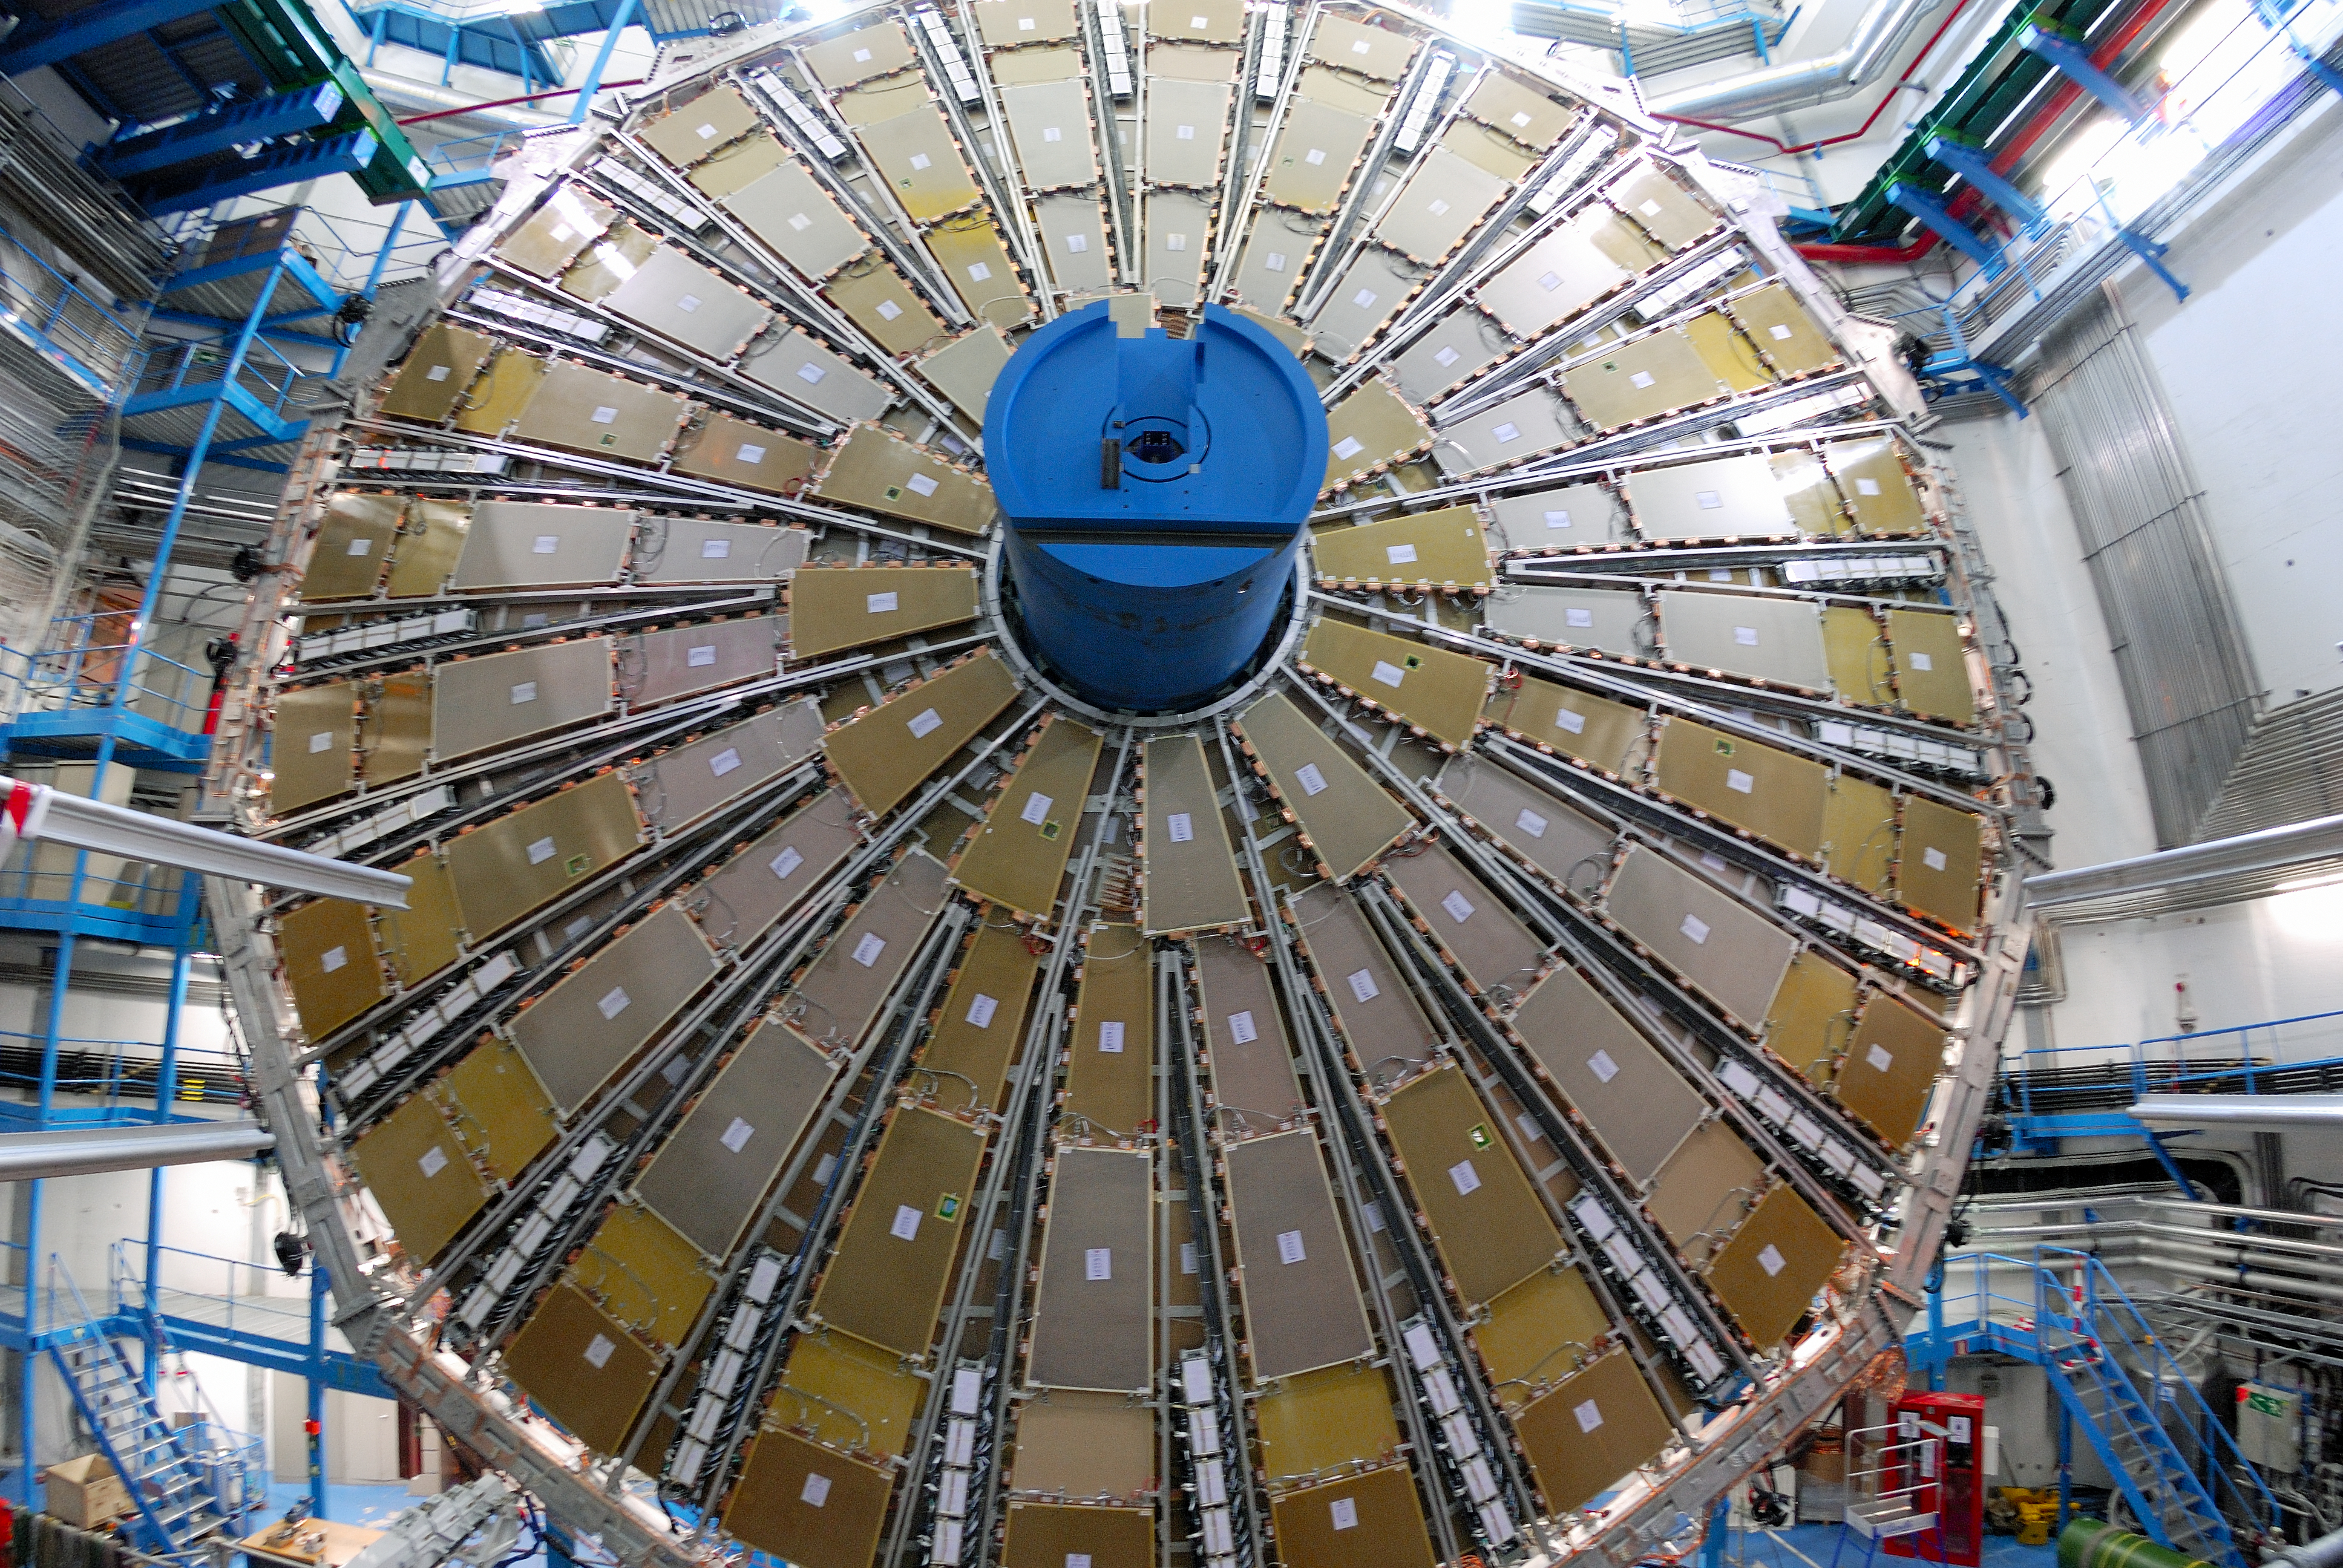
\includegraphics[width=0.8\textwidth]{figs/chapter2/TGC_pic.jpg}
  \caption{The picture of one side of TGC BW, including 24 sectors along $\phi$ direction.\cite{TGCInstallation}.}
  \label{fig:TGC_pic}
\end{figure}

TGCs are multi-wire proportional chambers (MWPCs), as illustrated in Figure~\ref{fig:TGC_cross_section}. The chamber contains \textit{wires} and \textit{strips}, which are arranged orthogonally to enable a two-dimensional readout. As the name suggests, the \textit{wire segments}, which include the sense wires, provide measurement in $R$ direction, while the \textit{strip segments} correspond to the $\phi$ direction. The chambers are filled with a gas mixture of CO$_2$ and n-C$_5$H$_{12}$, with a high voltage of 2.8~kV applied to the wires. To achieve bunch crossing identification every 25~ns, which is corresponding to the bunch crossing frequency of 40~MHz, the system requires high time resolution. Therefore, the wire spacing is 1.8~mm, and the wire-strip spacing is 1.4~mm to reduce drift time and signal readout delay.

\begin{figure}[htbp]
  \centering
  \includegraphics[width=0.7\textwidth]{figs/chapter2/TGC_cross_section.png}
  \caption{The structure of TGC, including anode wires, graphite cathodes, G-10 layers and a pick-up strip, orthogonal to the wires.\cite{ATLASDetector2008}.}
  \label{fig:TGC_cross_section}
\end{figure}

For higher space resolution during reconstruction, stations are composed of multiple layers. M1 contains three layers of wires and two layers of strips (\textit{triplet}), while M2 and M3 consist of two layers each for both wires and strips (\textit{doublet}). These layers are all ``staggered'' intentionally with adjacent layers, generating the conception of \textit{staggered ID}, which indicates the coincidence result of Intra Station Coincidence within segments. Each staggered ID corresponds to a unique channel combination that spans across offset wire or strip layers, and enables finer position resolution than the raw layer granularity. For example, in M1 with three wire layers staggered by 1/3 each, the staggered ID achieves roughly 1/3 of the layer's intrinsic spatial resolution. In M2 and M3, the two-layer structure results in a resolution gain of roughly 1/2 per ID unit. The staggered IDs are systematically defined and registered in databases, allowing consistent identification and grouping of segments across layers during pattern recognition and offline reconstruction. An illustration of the channel-staggered IDs correspindence table are given as Figure~\ref{fig:staggeredID}.

\begin{figure}[htbp]
  \centering
  \includegraphics[width=0.9\textwidth]{figs/chapter2/staggeredID.png}
  \caption{Correspondence table between channel number and staggered ID, Illustrated of the endcap wire segment.}
  \label{fig:staggeredID}
\end{figure}

%====================================================================================================
\section{TDAQ System} \label{sec:TDAQSystem}
%====================================================================================================


\clearpage
%====================================================================================================
\section{Upgrade for Muon Spectrometer} \label{sec:MuonUpgrade}
%====================================================================================================

%====================================================================================================
\section{Upgrade for TDAQ System} \label{sec:TDAQUpgrade}
%====================================================================================================
